\documentclass[12pt, a4paper]{article} 
\usepackage{tcolorbox}
\tcbuselibrary{skins, breakable, theorems}
\usepackage{subcaption}
\usepackage{pdflscape} 

\newtcbtheorem{question}{题~(理}%
  {enhanced, breakable,
    colback = white, colframe = cyan, colbacktitle = cyan,
    attach boxed title to top left = {yshift = -2mm, xshift = 5mm},
    boxed title style = {sharp corners},
    fonttitle = \sffamily\bfseries, separator sign = {).~}}{qst}
\input{pre._CJK_thesis}   % 使用自己維護的定義檔
%-----------------------------------------------------------------------------------------------------------------------
% 文章開始
\title{ Teps-b資料統計}
\author{{\SM 鄭仲恒}}
\date{{\TT \today}} 	 
\begin{document}
\maketitle
\fontsize{12}{22 pt}\selectfont
Teps-b統計資料與圖形分析,CP代表原先調查為國中生族群,SH為原先調查高中生族群。文章先由CP核心資料先介紹,再後續介紹SH。

%%%%%%%%%%%%%%%%%%%%%%%%%%%%


\section{CP-核心資料國中生}
調查的資料分佈年份為2009、2013、2014、2019年,其中2014年度為專員實際進行面訪受訪者,其餘3次調查譏為電話訪談資料。
\subsection{2009年度調查-電訪}
變數資料經行統整,其中針對部分變數進行合併,重新標籤。

\begin{table}[htbp]
  \centering
   \caption{2009CP-樣本性別}
  \begin{adjustbox}{width=0.5\textwidth}
    \begin{tabular}{lcccc}
      \toprule
      TEPS-B & 樣本性別 & Freq. & Percent & Cum. \\
      \midrule
      & 男 & 1,764 & 49.10 & 49.10 \\
      & 女 & 1,829 & 50.90 & 100.00 \\
      \midrule
      Total & & 3,593 & 100.00 & \\
      \bottomrule
    \end{tabular}
  \end{adjustbox}
\end{table}

\bigskip

\begin{table}[htbp]
  \centering
  \caption{性別與學校類別}
  \begin{adjustbox}{width=\textwidth}
    \begin{tabular}{lcccccccccc}
      \toprule
      TEPS-B & 樣本性 & 大學 & 私立大學 & 國立科技 & 私立科技 & 技職學院 & 學院 & 國外大學 & 遺漏 & 跳答 \\
      \midrule
      & 男 & 424 & 528 & 100 & 256 & 150 & 16 & 9 & 178 & 103 \\
      & 女 & 350 & 639 & 77 & 247 & 162 & 8 & 25 & 230 & 91 \\
      \midrule
      Total & & 774 & 1,167 & 177 & 503 & 312 & 24 & 34 & 408 & 194 \\
      \bottomrule
    \end{tabular}
  \end{adjustbox}
\end{table}


\begin{figure}[h]
    \centering    
        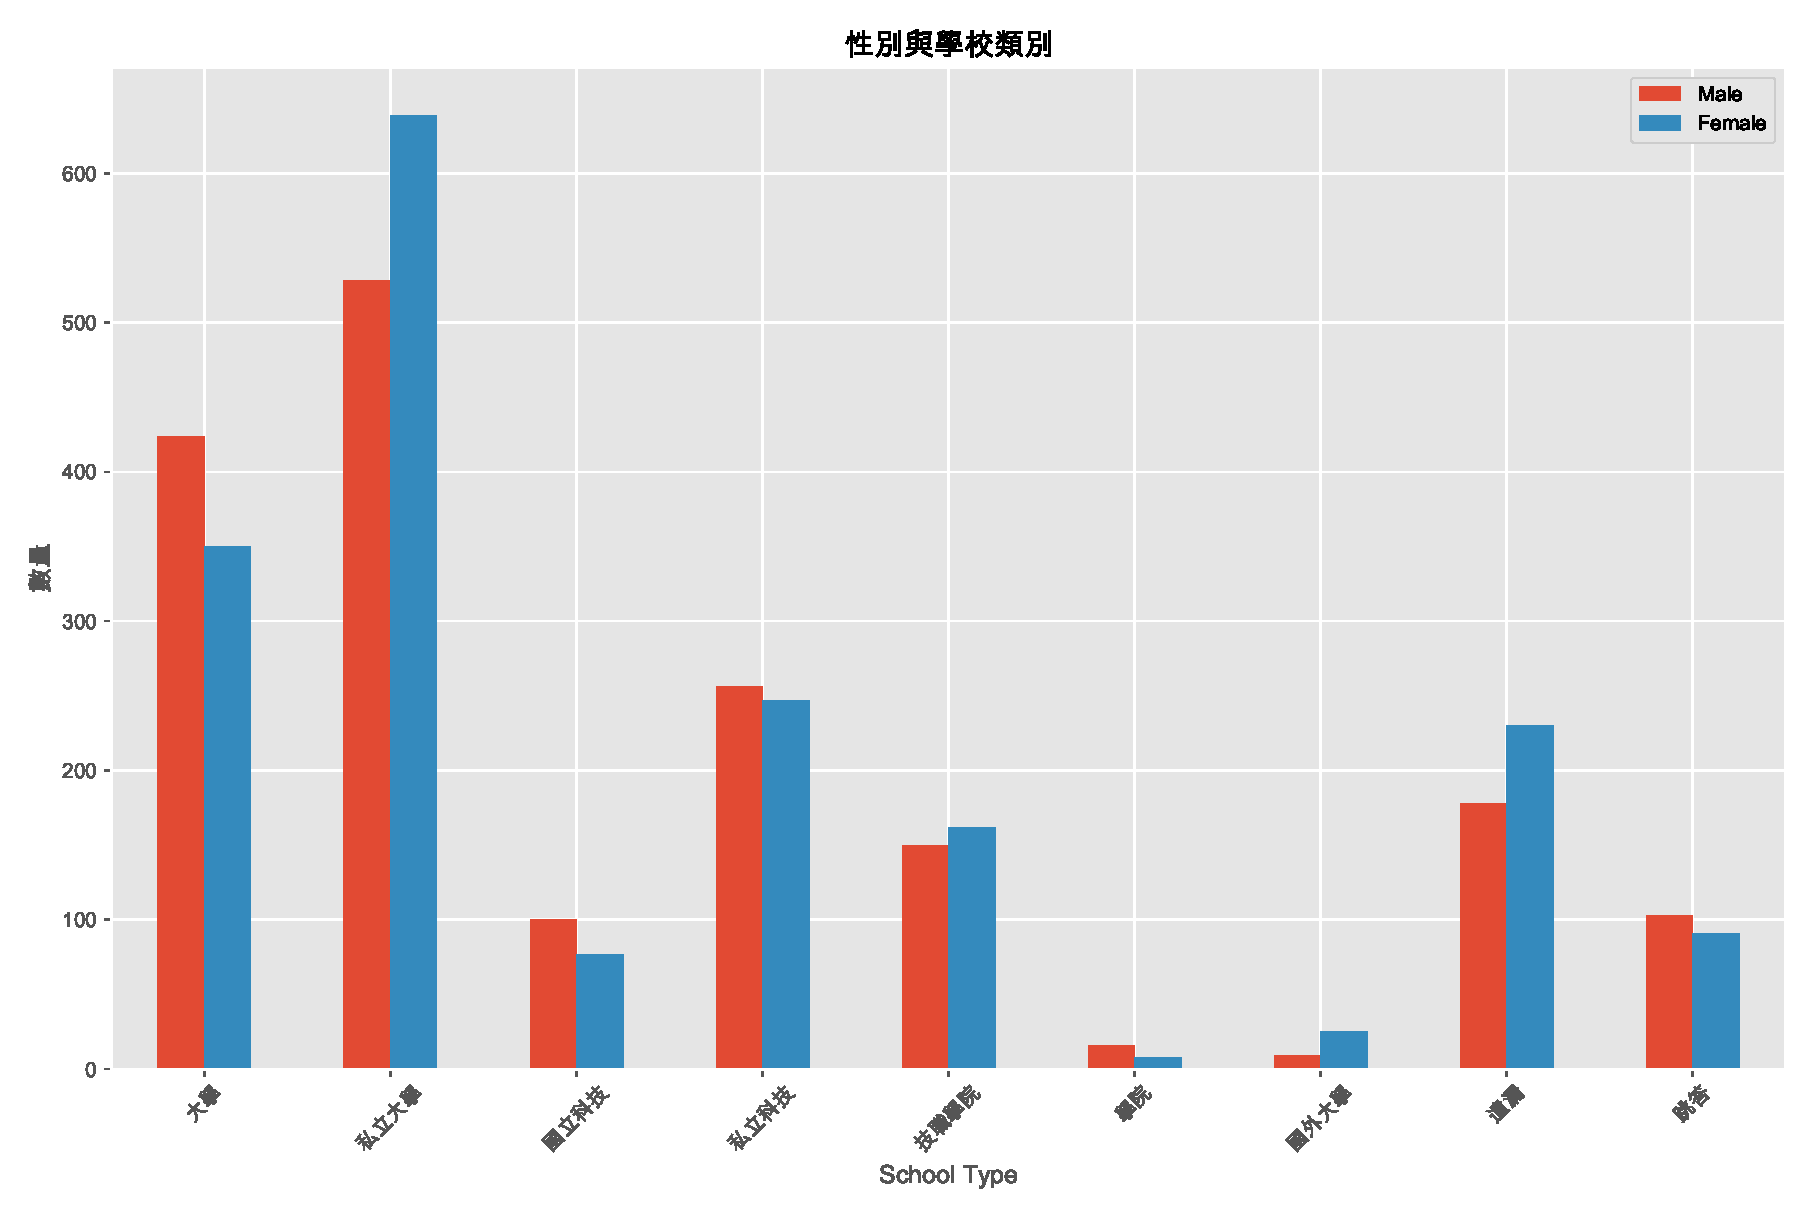
\includegraphics[width=\linewidth]{\imgdir/gender_school.eps}
        \caption{學校種類與薪酬}
        \label{pic:學校種類與薪酬}
\end{figure}









\begin{table}[ht]
\centering
\renewcommand{\arraystretch}{1.3} %%%把表格的高拉大
\extrarowheight=4pt
\caption{原始資料學歷與工作經驗}
\begin{adjustbox}{width=\textwidth}
\begin{tabular}{l*{8}{c}}
\toprule
& \multicolumn{8}{c}{受訪者工作(針對第一份工作計算)} \\
\cmidrule(lr){2-9}
\multirow{2}{*}{大學學校分類} & \multirow{2}{*}{遺漏、跳答、不清楚} & \multirow{2}{*}{5年} & \multirow{2}{*}{4年-5年} & \multirow{2}{*}{3年-4年} & \multirow{2}{*}{2年-3年} & \multirow{2}{*}{1年-2年} & \multirow{2}{*}{1年內} & \multirow{2}{*}{Total} \\
& &  &  &  &  & &  &  \\
\midrule
公立一般大學 & 773 & 0 & 0 & 1 & 0 & 0 & 0 & 774 \\
公立一般學院 & 18 & 0 & 0 & 0 & 0 & 0 & 0 & 18 \\
公立科技大學 & 176 & 0 & 0 & 0 & 0 & 1 & 0 & 177 \\
公立技職學院 & 70 & 0 & 0 & 0 & 2 & 2 & 0 & 74 \\
公立專科學校 & 20 & 0 & 0 & 0 & 0 & 0 & 0 & 20 \\
私立一般大學 & 1,152 & 1 & 1 & 0 & 5 & 8 & 0 & 1,167 \\
私立一般學院 & 6 & 0 & 0 & 0 & 0 & 0 & 0 & 6 \\
私立科技大學 & 480 & 1 & 1 & 1 & 15 & 3 & 2 & 503 \\
私立技職學院 & 198 & 0 & 0 & 2 & 7 & 3 & 0 & 210 \\
私立專科學校 & 8 & 0 & 0 & 0 & 0 & 0 & 0 & 8 \\
國外大學 & 31 & 0 & 0 & 0 & 0 & 0 & 0 & 31 \\
其他 & 3 & 0 & 0 & 0 & 0 & 0 & 0 & 3 \\
遺漏值 & 397 & 0 & 0 & 0 & 0 & 0 & 0 & 397 \\
不知道、不清楚 & 4 & 0 & 0 & 0 & 0 & 0 & 0 & 4 \\
拒答 & 7 & 0 & 0 & 0 & 0 & 0 & 0 & 7 \\
跳答 & 159 & 0 & 0 & 3 & 25 & 4 & 3 & 194 \\
Total & 3,502 & 2 & 2 & 7 & 54 & 21 & 5 & 3,593 \\
\bottomrule
\end{tabular}
\end{adjustbox}

\end{table}



\begin{table}[ht]
\centering
\renewcommand{\arraystretch}{1.3} %%%把表格的高拉大
\extrarowheight=4pt
\caption{學歷經分類與工作經驗}
\begin{adjustbox}{width=\textwidth}
\begin{tabular}{l*{8}{c}}
\toprule
& \multicolumn{8}{c}{受訪者工作(針對第一份工作計算)} \\
\cmidrule(lr){2-9}
\multirow{2}{*}{大學學校種類} & \multirow{2}{*}{遺漏、跳答、不清楚} & \multirow{2}{*}{5年} & \multirow{2}{*}{4年-5年} & \multirow{2}{*}{3年-4年} & \multirow{2}{*}{2年-3年} & \multirow{2}{*}{1年-2年} & \multirow{2}{*}{1年內} & \multirow{2}{*}{Total} \\
& &  &  &  &  &  &  &  \\
\midrule
國立大學 & 773 & 0 & 0 & 1 & 0 & 0 & 0 & 774 \\
私立大學 & 1,152 & 1 & 1 & 0 & 5 & 8 & 0 & 1,167 \\
國立科技大學 & 176 & 0 & 0 & 0 & 0 & 1 & 0 & 177 \\
私立科技大學 & 480 & 1 & 1 & 1 & 15 & 3 & 2 & 503 \\
技職學院、專科學校 & 296 & 0 & 0 & 2 & 9 & 5 & 0 & 312 \\
學院 & 24 & 0 & 0 & 0 & 0 & 0 & 0 & 24 \\
國外大學、其他 & 34 & 0 & 0 & 0 & 0 & 0 & 0 & 34 \\
遺漏、不清楚、拒答 & 408 & 0 & 0 & 0 & 0 & 0 & 0 & 408 \\
跳答 & 159 & 0 & 0 & 3 & 25 & 4 & 3 & 194 \\
Total & 3,502 & 2 & 2 & 7 & 54 & 21 & 5 & 3,593 \\
\bottomrule
\end{tabular}
\end{adjustbox}
\end{table}



\begin{figure}[H]
    \centering    
        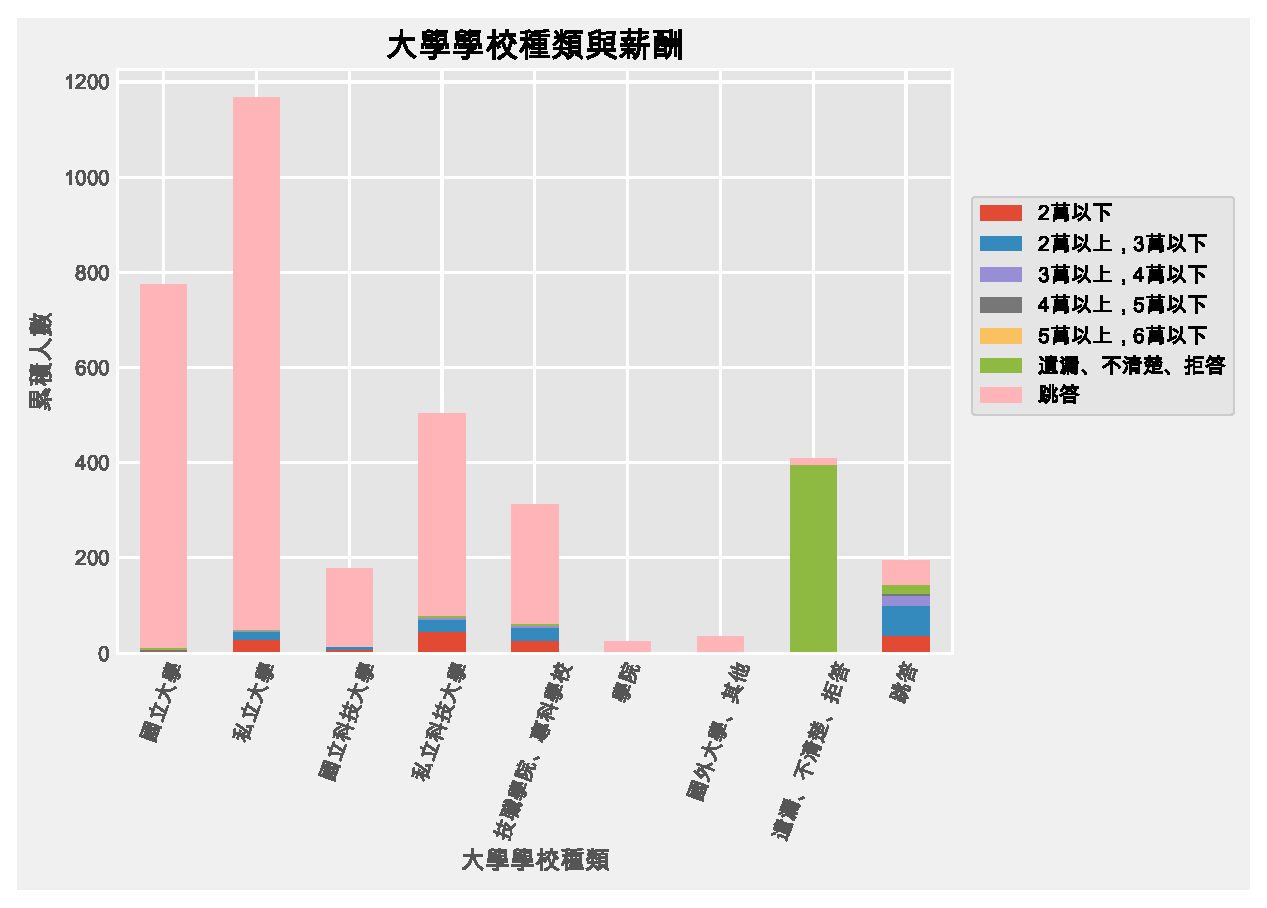
\includegraphics[width=\linewidth]{\imgdir/school_type_salary.eps}
        \caption{學校種類與薪酬}
        \label{pic:學校種類與薪酬}
\end{figure}

\begin{table}[ht]
\centering
\renewcommand{\arraystretch}{1.3} %%%把表格的高拉大
\extrarowheight=4pt
\begin{adjustbox}{width=\textwidth}
\begin{tabular}{l*{8}{c}}
\toprule
& \multicolumn{8}{c}{薪酬經過重新分組} \\
\cmidrule(lr){2-9}
大學學校種類 & 2萬以下 & 2萬以上& 3萬以上 & 4萬以上 & 5萬以上 & 遺漏、 & 跳答 & Total \\
		   &    &-3萬以下    & -4萬以下  &- 5萬以下    & -6萬以下   & 不清楚、拒答   &   &  \\
\midrule
國立大學 & 5 & 3 & 0 & 0 & 0 & 3 & 763 & 774 \\
私立大學 & 28 & 17 & 2 & 0 & 0 & 2 & 1,118 & 1,167 \\
國立科技大學 & 7 & 6 & 0 & 0 & 0 & 1 & 163 & 177 \\
私立科技大學 & 46 & 24 & 4 & 0 & 0 & 6 & 423 & 503 \\
技職學院、專科學校 & 27 & 27 & 4 & 0 & 1 & 3 & 250 & 312 \\
學院 & 0 & 1 & 0 & 0 & 0 & 0 & 23 & 24 \\
國外大學、其他 & 0 & 0 & 0 & 0 & 0 & 0 & 34 & 34 \\
遺漏、不清楚、拒答 & 1 & 1 & 0 & 0 & 0 & 395 & 11 & 408 \\
跳答 & 37 & 62 & 23 & 3 & 1 & 18 & 50 & 194 \\
Total & 151 & 141 & 33 & 3 & 2 & 428 & 2,835 & 3,593 \\
\bottomrule
\end{tabular}
\end{adjustbox}
\caption{薪酬經過重新分組的表格}
\end{table}








\end{document}
